\section{Results}
\label{sec:results}

% \akshita{following rewrites in Method section, we can now simply move up the ablations table here and report all results. we can also move up some of the discussion from Ablating section here combining it with the results discussed here -- it can be more a comparison of choices for each task, rather than talking in terms of average error for each feature}. 

%\begin{figure*}[t]
\small
\setlength{\tabcolsep}{3pt}
\centering
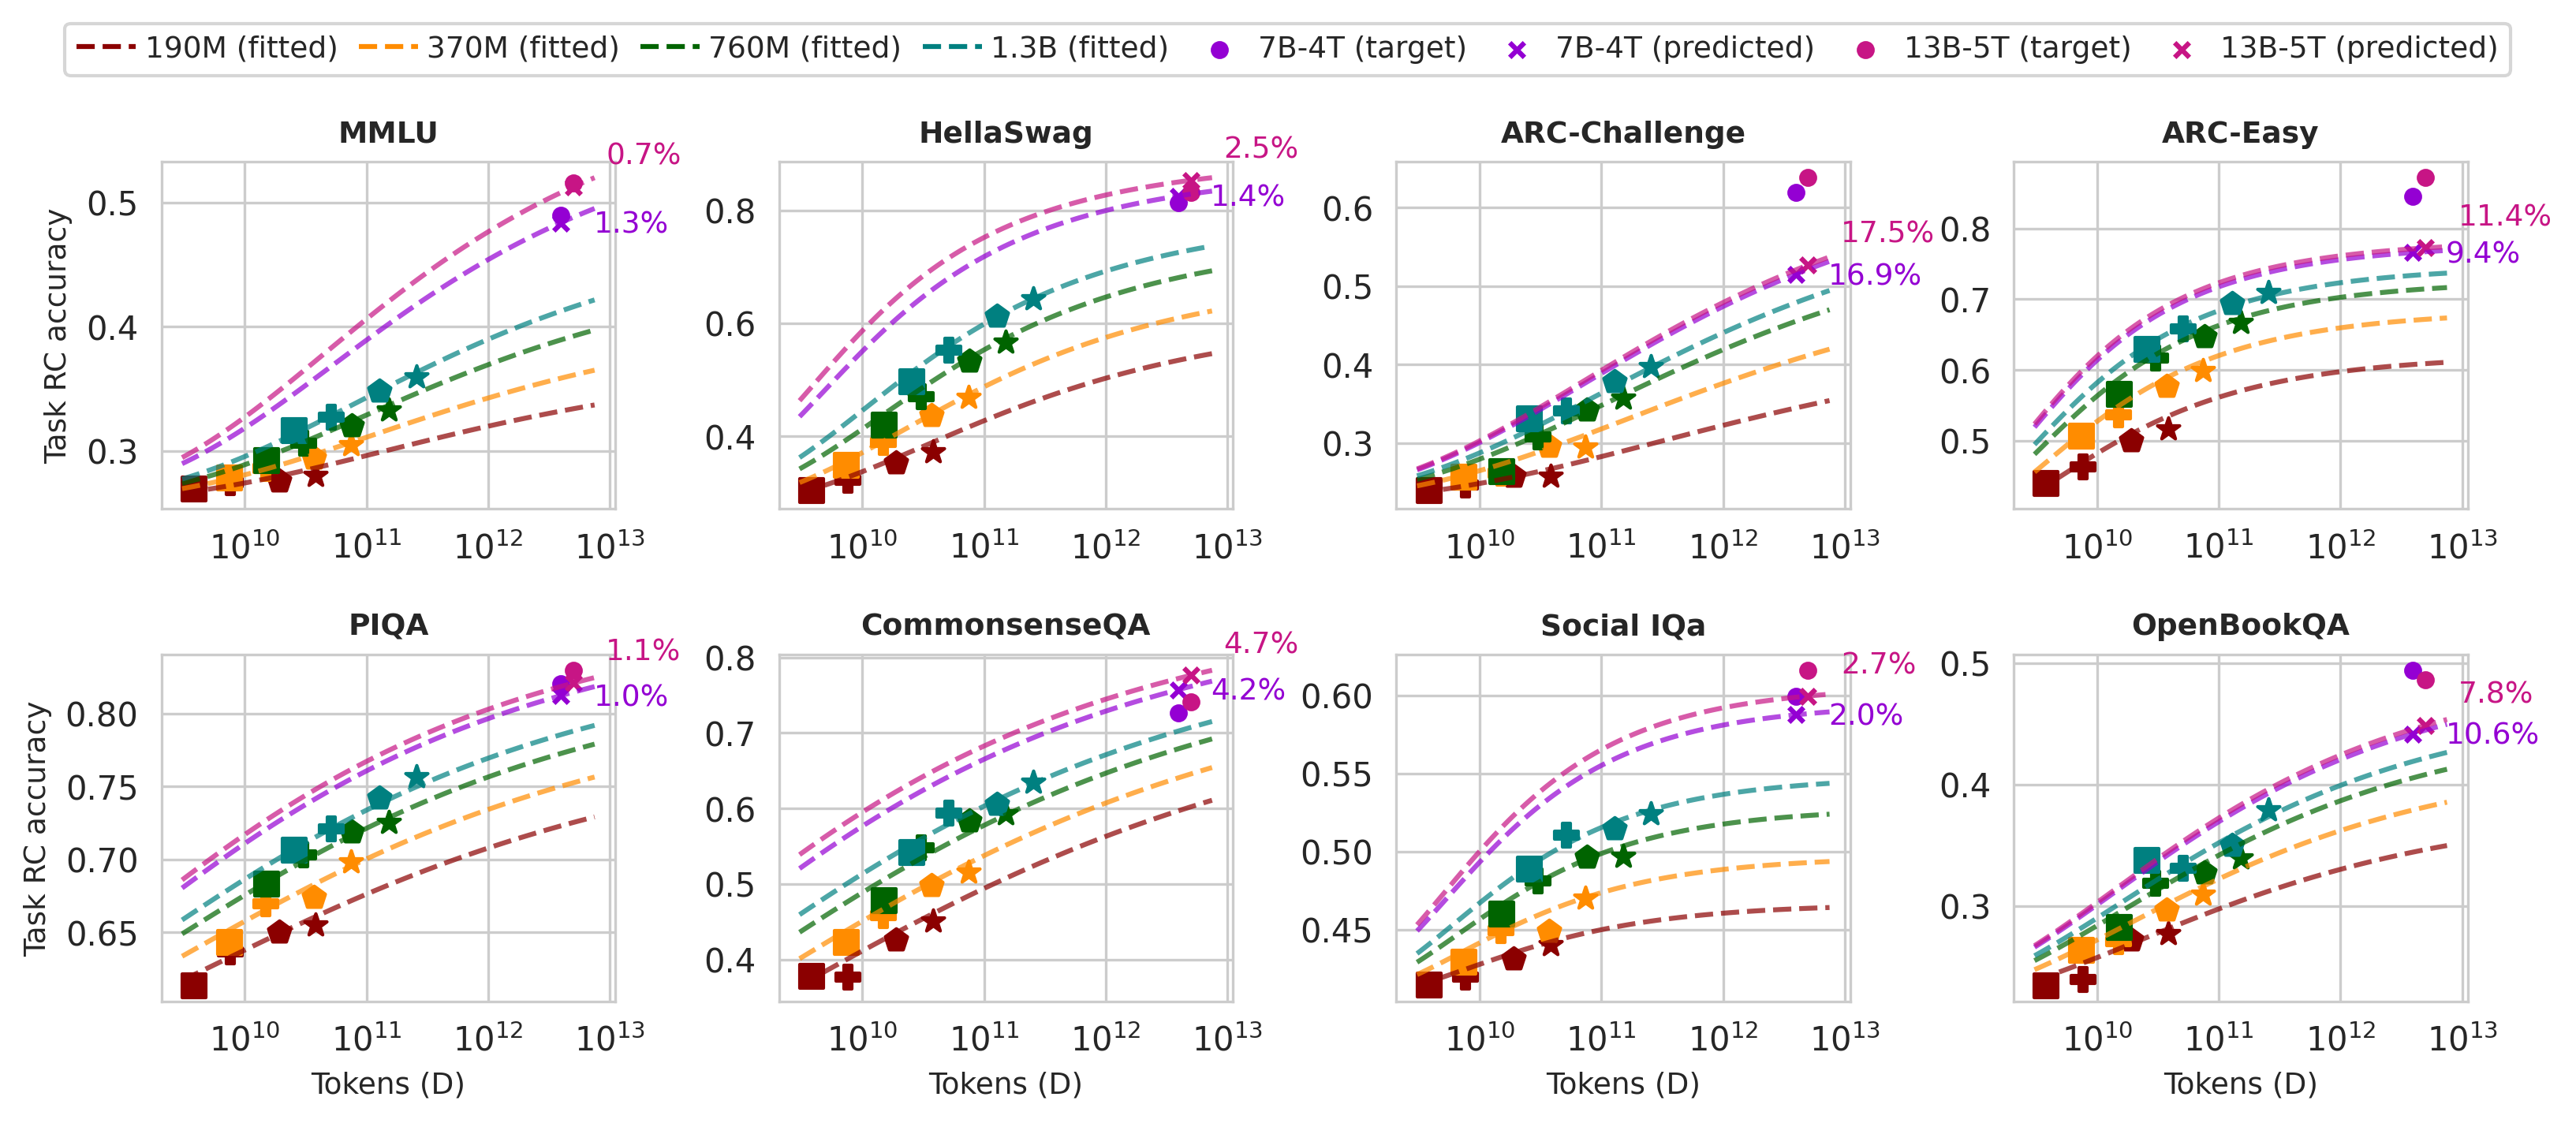
\includegraphics[scale=0.5]{images/chained_main.png}
\resizebox{0.75 \textwidth}{!}{%
\begin{tabular}{l c r | r r r r | r r r r}
\toprule
& & & \multicolumn{4}{c}{\textbf{7B-4T}} & \multicolumn{4}{c}{\textbf{13B-5T}}\\
\textbf{Task} & \textbf{Split} & \textbf{Examples} & Pred & Actual & Error & \%Error & Pred & Actual & Error & \%Error \\
\midrule
MMLU & test & 14,042 & 48.4 & 49.0 & 0.6 & 1.3\% & 51.3 & 51.6 & 0.3 & 0.7\% \\
HellaSwag & val & 10,042 & 82.5 & 81.3 & 1.2 & 1.4\% & 85.3 & 83.2 & 2.1 & 2.5\% \\
ARC-Challenge & test & 1,172 & 51.5 & 61.9 & 10.4 & 16.9\% & 52.7 & 63.8 & 11.1 & 17.5\% \\
ARC-Easy & test & 2,376 & 76.6 & 84.6 & 8.0 & 9.4\% & 77.2 & 87.2 & 10.0 & 11.4\% \\
PIQA & val & 1,838 & 81.2 & 82.0 & 0.8 & 1.0\% & 82.1 & 83.0 & 0.9 & 1.1\% \\
CommonsenseQA & val & 1,221 & 75.7 & 72.6 & 3.1 & 4.2\% & 77.6 & 74.1 & 3.5 & 4.7\% \\
Social IQa & val & 1,954 & 58.7 & 59.9 & 1.2 & 2.0\% & 59.9 & 61.6 & 1.7 & 2.7\% \\
OpenBookQA & test & 500 & 44.2 & 49.4 & 5.2 & 10.6\% & 44.9 & 48.6 & 3.7 & 7.8\% \\
\midrule
Average & -- & -- & -- & -- & 3.8 & 5.9\% & -- & -- & 4.2 & 6.1\% \\
\bottomrule
\end{tabular}
}%
\caption{
Task accuracy prediction for the target models using task loss as the intermediate feature.
\ding{110} = 1xC; \ding{58} = 2xC; $\pentagofill$ = 5xC; $\bigstar$ = 10xC.
Prediction error is next to the target.
}
\label{tab:stacked_pred}
\vspace{-8pt}
\end{figure*}


\begin{table*}[t]
\small
\setlength{\tabcolsep}{2pt}
\centering
\caption{
Comparison of design choices.
\textbf{Upper:} Average step 1 prediction error.
\textbf{Lower:} Average chained prediction error. For MMLU, using task loss yields the lowest prediction error. We observe higher errors for ARC-C, ARC-E, and OBQA with task loss, which aligns with our variance analysis in \S\ref{sec_variance_analysis}, and that C4 as the intermediate loss works better for them.
}
\resizebox{1.0 \textwidth}{!}{%
\begin{tabular}{l | c c c c c c c c | c c c c c c c c}
\toprule
& \multicolumn{8}{c}{\textbf{7B-4T}} & \multicolumn{8}{c}{\textbf{13B-5T}} \\
\textbf{Design choice} & \textbf{MMLU} & \textbf{HS} & \textbf{ARC-C} & \textbf{ARC-E} & \textbf{PIQA} & \textbf{CSQA} & \textbf{SIQa} & 
\textbf{OBQA} & \textbf{MMLU} & \textbf{HS} & \textbf{ARC-C} & \textbf{ARC-E} & \textbf{PIQA} & \textbf{CSQA} & \textbf{SIQa} & 
\textbf{OBQA} \\
\midrule
(N, D) $\rightarrow$ task loss (\S\ref{sec:method}) & 1.3\% & 0.3\% & 7.0\% & 13.3\% & 2.0\% & 11.7\% & 4.3\% & 1.3\% & 0.2\% & 1.2\% & 9.4\% & 16.0\% & 2.7\% & 18.5\% & 3.6\% & 0.9\% \\
\midrule
FLOPs $\rightarrow$ task loss (\S\ref{app:flops_as_feature}) & 4.3\% & 2.1\% & 2.4\% & 5.3\% & 2.0\% & 12.5\% & 5.7\% & 0.5\% & 5.2\% & 2.6\% & 3.5\% & 7.0\% & 2.6\% & 18.8\% & 5.7\% & 1.4\% \\
\bottomrule
\end{tabular}
}%
\vspace{4pt}
\resizebox{1.0 \textwidth}{!}{%
\begin{tabular}{l | c c c c c c c c | c c c c c c c c}
\toprule
& \multicolumn{8}{c}{\textbf{7B-4T}} & \multicolumn{8}{c}{\textbf{13B-5T}} \\
\textbf{Design choice} & \textbf{MMLU} & \textbf{HS} & \textbf{ARC-C} & \textbf{ARC-E} & \textbf{PIQA} & \textbf{CSQA} & \textbf{SIQa} & 
\textbf{OBQA} & \textbf{MMLU} & \textbf{HS} & \textbf{ARC-C} & \textbf{ARC-E} & \textbf{PIQA} & \textbf{CSQA} & \textbf{SIQa} & 
\textbf{OBQA} \\
\midrule
(N, D) $\rightarrow$ task loss (\S\ref{sec:method}) & \textbf{1.3\%} & 1.4\% & 16.9\% & 9.4\% & 1.0\% & 4.2\% & 2.0\% & 10.6\% & \textbf{0.7\%} & 2.5\% & 17.5\% & 11.4\% & 1.1\% & 4.7\% & 2.7\% & 7.8\% \\
\midrule
TaskCE (\S\ref{app:task_ce}) & 18.3\% & 7.2\% & 21.3\% & 5.4\% & 3.1\% & \textbf{2.6\%} & \textbf{0.7\%} & 7.1\% & 20.2\% & 10.5\% & 19.5\% & 6.2\% & 2.9\% & \textbf{2.7\%} & \textbf{1.2\%} & \textbf{0.2\%} \\
C4 loss (\S\ref{app:c4}) & 2.2\% & 4.5\% & \textbf{1.4\%} & \textbf{1.2\%} & \textbf{0.7\%} & 5.8\% & 6.2\% & \textbf{2.0\%} & 5.0\% & 5.7\% & \textbf{3.9\%} & \textbf{1.9\%} & 1.5\% & 7.0\% & 7.6\% & 10.4\% \\
Single step (\S\ref{app:single_step}) & 5.6\% & \textbf{0.5\%} & 21.7\% & 6.1\% & \textbf{0.7\%} & 5.1\% & 5.4\% & 9.0\% & 7.1\% & \textbf{0.8\%} & 22.6\% & 7.9\% & \textbf{0.6\%} & 6.6\% & 6.8\% & 4.7\% \\
\bottomrule
\end{tabular}
}%
\label{tab:design_choices}
\vspace{-8pt}
\end{table*}

% \begin{table*}[t]
% \small
% \setlength{\tabcolsep}{3pt}
% \centering
% \caption{
% \textbf{ Comparison of design choices}: 
% }
% \vspace{-12pt}
% \end{table*}


\autoref{tab:design_choices} compares prediction errors for all design choices. 

\tightparagraph{Task loss.}
\autoref{tab:stacked_pred} shows the chained prediction results on the target models using task loss as the intermediate feature.
On four tasks -- MMLU, HellaSwag, PIQA, and Social IQa -- we predict the accuracy within an absolute error of 2 points.
For ARC-C and ARC-E, we overestimate the task loss in step 1, and underestimate the task accuracy in step 2. In \S\ref{sec_variance_analysis}, we analyze the ability of the ladder to predict task performance by considering variation between checkpoints. We find that our results here track with the variation analysis (ARC-E and ARC-C display higher variance).

%For task loss, we also report predictions for the 32B model size in \autoref{tab:stacked_preds_32b}. The predictions are within an absolute error of 3 points on tasks like HellaSwag, PIQA, and Social IQA (similar to the predictions for 7B and 13B models). 

\tightparagraph{TaskCE.}
Using TaskCE as the intermediate feature results in overall higher prediction errors for several tasks (including MMLU and HellaSwag; see \S\ref{sec:ablations} on why these tasks are especially important). Full results using TaskCE are shown in \S\ref{app:task_ce}.

\tightparagraph{LM loss.}
Interestingly, the loss on C4-en validation set is a good predictor of task accuracy for several tasks. One possible explanation for this is potential domain overlap between the task and the validation set. We discuss pros and cons of using LM loss in \S\ref{sec:ablations}. Full results using LM Loss are show in \S\ref{app:c4}.

Figure \ref{fig:intermediate_feature_comparison} compares absolute and relative errors for all three intermediate features.

%\begin{figure*}[t]
\small
\setlength{\tabcolsep}{3pt}
\centering
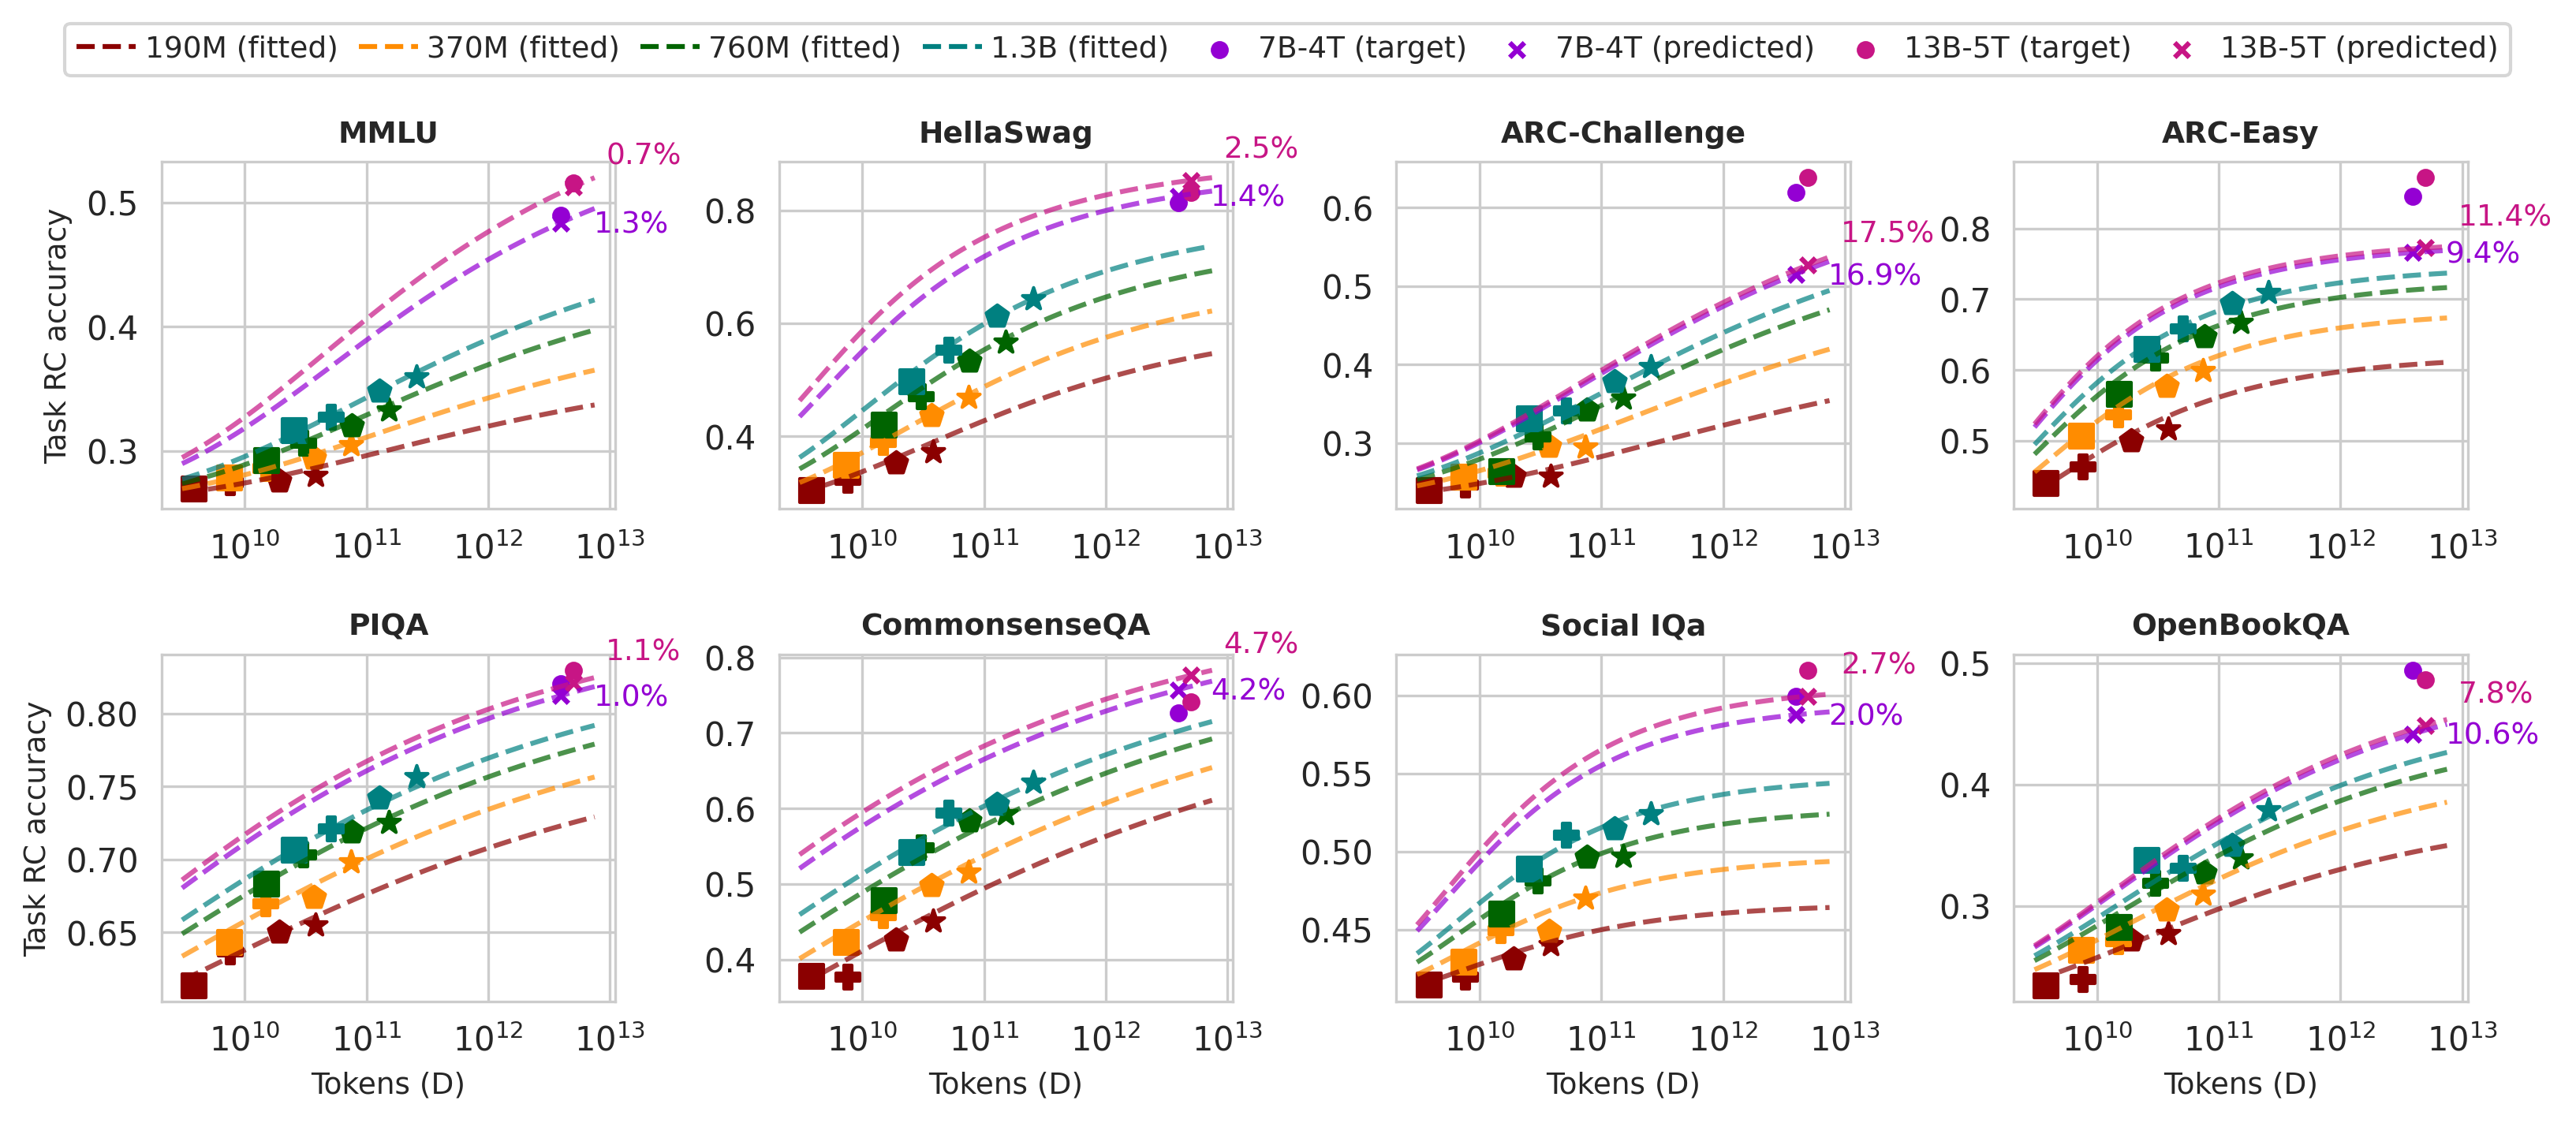
\includegraphics[scale=0.5]{images/chained_main.png}
\resizebox{0.75 \textwidth}{!}{%
\begin{tabular}{l | r r r r}
\toprule
& \multicolumn{4}{c}{\textbf{32B-6T}} \\
\textbf{Task} & Pred & Actual & Error & \%Error \\
\midrule
%MMLU & 48.4 & 49.0 & 0.6 & 1.3\%  \\
HellaSwag & 88.0 & 85.3 & 2.7 & 3.07\% \\
ARC-Challenge & 53.6 & 66.8 & 13.2 & 24.63\% \\
ARC-Easy & 77.8 & 88.8 & 11.0 & 14.14\% \\
PIQA & 82.9 & 83.6 & 0.7 & 0.84\% \\
CommonsenseQA & 79.5 & 75.4 & 4.1 & 5.16\% \\
Social IQa & 61.1 & 62.3 & 1.2 & 1.96\% \\
OpenBookQA & 45.4 & 53.2 & 7.8 & 17.18\% \\
\midrule
Average & -- & -- & 5.81 & 9.57\% \\
\bottomrule
\end{tabular}
}%
\caption{
Task accuracy prediction for the 32B model using task loss as the intermediate feature.
\ding{110} = 1xC; \ding{58} = 2xC; $\pentagofill$ = 5xC; $\bigstar$ = 10xC.
Prediction error is next to the target.}
\label{tab:stacked_preds_32b}
\vspace{-8pt}
\end{figure*}

% Task	Pred	Actual
% HellaSwag	88.0	85.3
% ARC-Challenge	53.6	66.8
% ARC-Easy	77.8	88.8
% PIQA	82.9	83.6
% CSQA	79.5	75.4
% Social IQA	61.1	62.3
% OpenBookQA	45.4	53.2

% There are several factors to explain this:

% \tightparagraph{Predictive power of the intermediate feature}.
% Tasks with noisy mapping between their inter


% Using task loss to predict accuracy has low error for MMLU, PIQA, HellaSwag, and Social IQa, corresponding to the tasks with the lowest variance around task loss and accuracy, as observed in \autoref{tab:variance_analysis}.

% Tasks with a noisy mapping between their intermediate feature and accuracy (e.g., ARC-Challenge, ARC-Easy and OpenBookQA) may have compounded errors in the two-step prediction. 
% This may explain the higher prediction errors for the design choices which directly or indirectly rely on an intermediate representation of the task loss. For ARC-Challenge and OpenBookQA in particular, their high variance for both the intermediate task loss and accuracy make them challenging to predict with the ladder. 
% HellaSwag and PIQA, the tasks where we observe the least variance, are the easiest to predict across all design choices, including the combined single step approach. 

% Finally, MMLU and HellaSwag have large sample sizes -- 5x larger than the other tasks in this work. Given their low sample variance and noise around the prediction target, we expect their errors are most representative of the true difficulty of predicting downstream performance. Thus, we present the two-step prediction as our main approach.

% \tightparagraph{Step 1 results.}
% \autoref{fig:step1} shows the function fitting of step 1 on the ladder models, and the prediction of task loss for the target models.
% The function gives an average relative \textit{fitting error} ranging from 0.2\% to 1.2\%, which suggests that \autoref{eqn:power} is a good functional form to describe task losses.
% We have a relative \textit{prediction error} within 3\% on MMLU, HellaSwag, PIQA, and OpenBookQA.
% Our method underestimates the loss for CSQA, and overestimates on ARC-Challenge, ARC-Easy, and Social IQa.

%Overestimating the task loss can lead us to eventually underestimate the task accuracy. 

%\begin{figure*}[t]
\centering
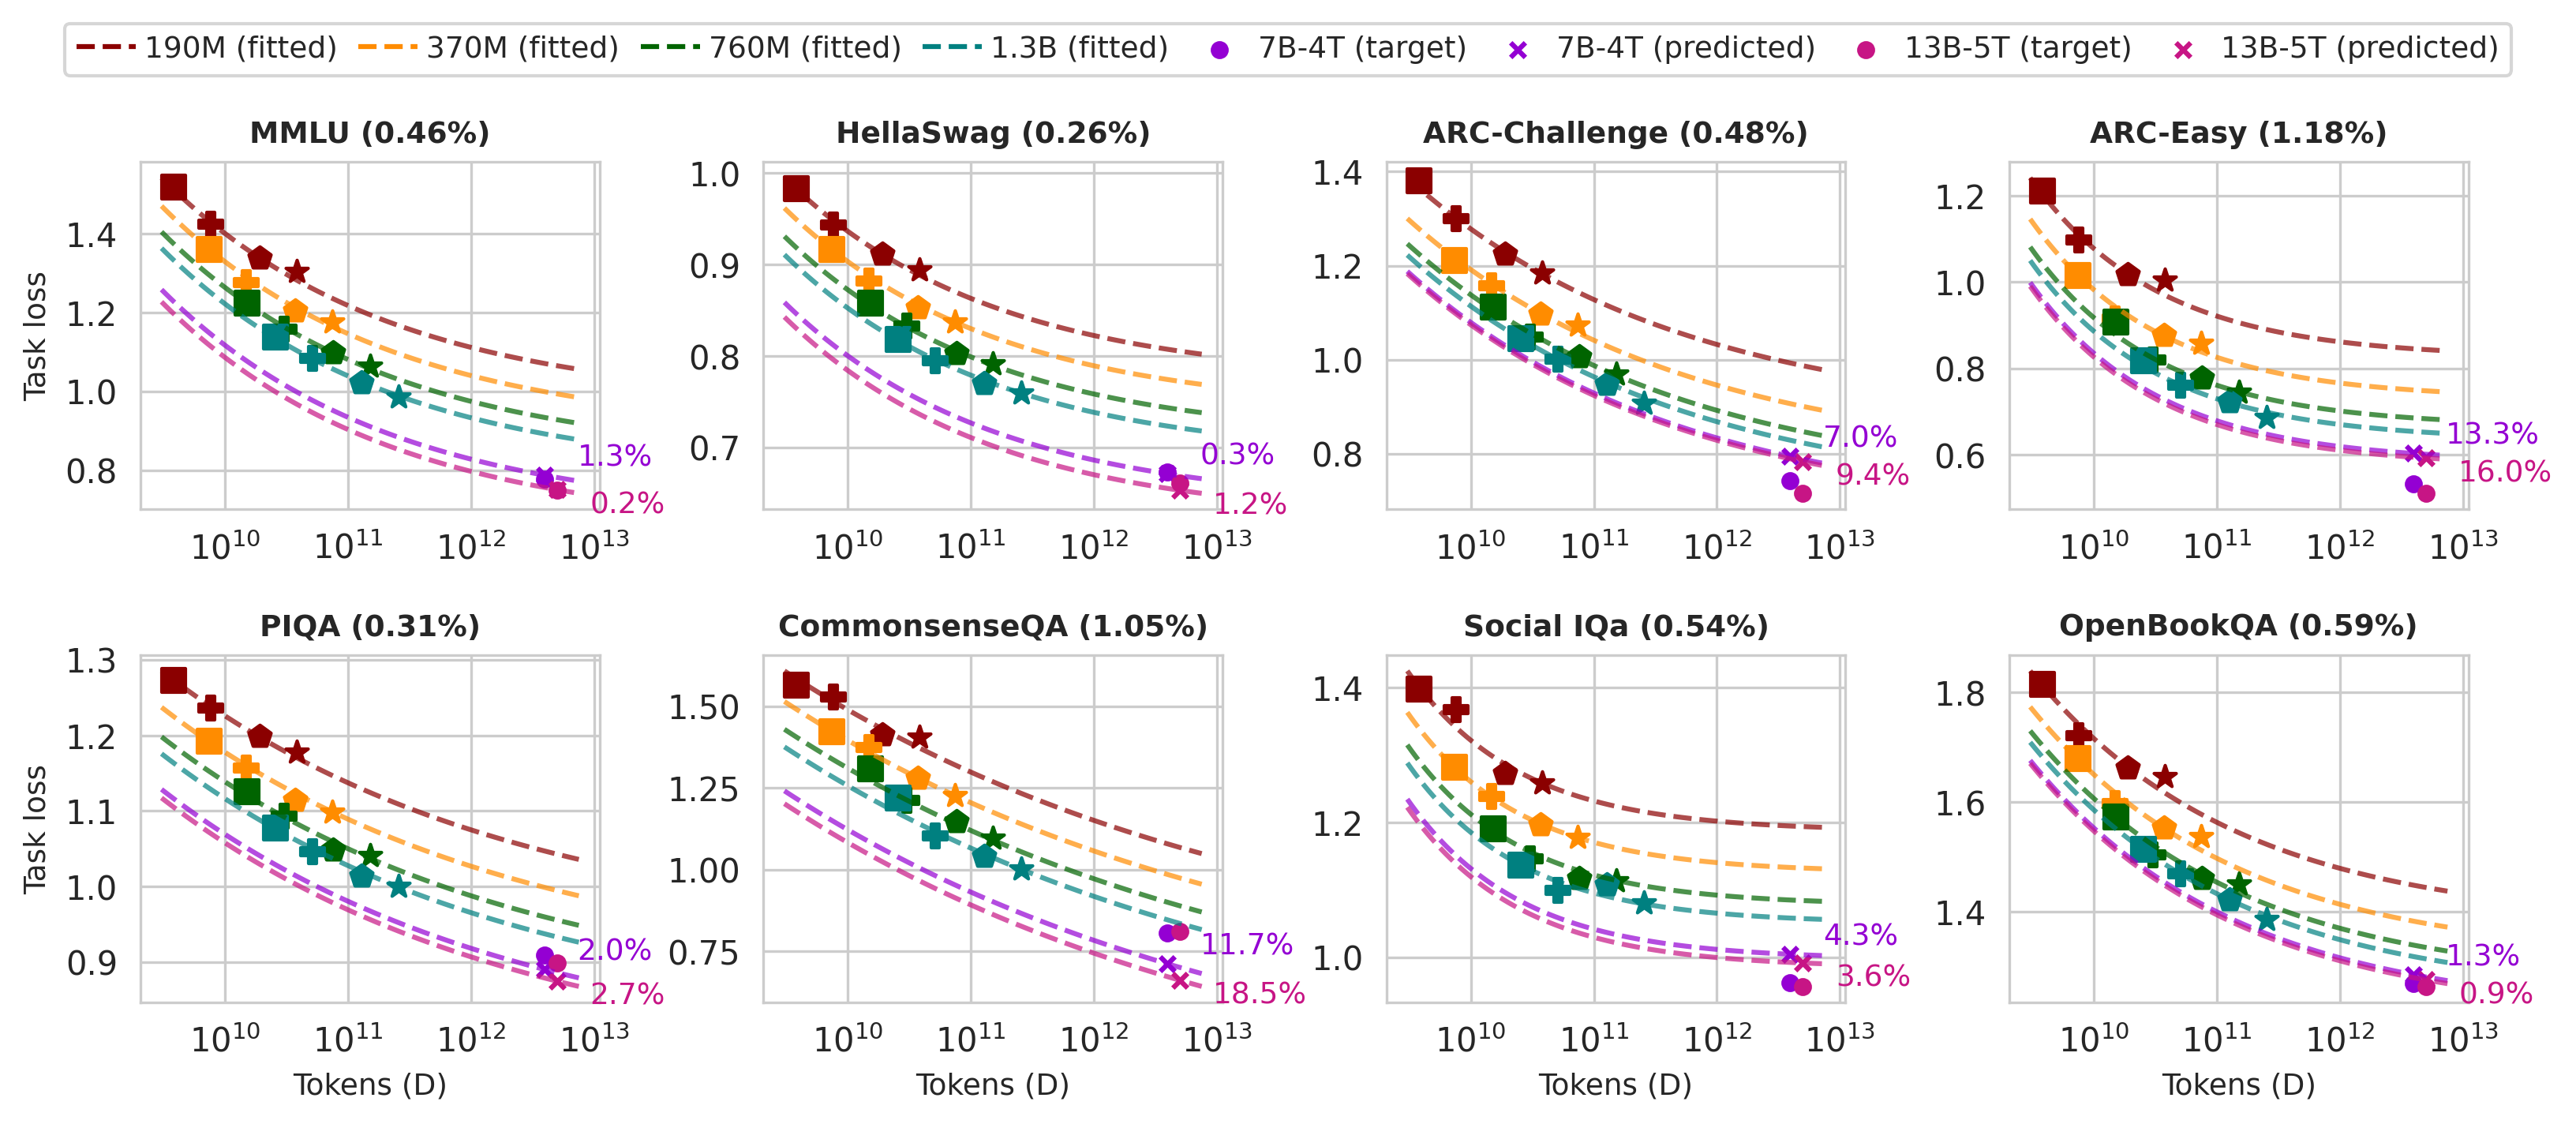
\includegraphics[width=\linewidth]{images/step1_main.png}
\vspace{-16pt}
\caption{
    Task loss vs training scale $(N, D)$, with fitting on the power function in \autoref{eqn:power}.
    \ding{110} = 1xC; \ding{58} = 2xC; $\pentagofill$ = 5xC; $\bigstar$ = 10xC.
    We report the average relative fitting error in parentheses after the task name, and prediction error next to the target model point.
    %In general, the power function fits well to data points from the ladder models, and the fitted function makes rather reliable predictions for the targer models.
    %See \autoref{tab:fitted_params} for the parameters of the fitted functions.
}
\label{fig:step1}
\vspace{-8pt}
\end{figure*}

% \tightparagraph{Step 2 results.}
% \autoref{fig:step2} shows the function fitting of step 2 on the ladder models, and the prediction of task accuracy for the target models with their \textit{actual} task loss.
% For all tasks, all data points fit well with a shared sigmoidal function, with the average relative \textit{fitting error} ranging from 0.4\% to 2.6\%.
% We get within 3\% relative \textit{prediction error} on MMLU, HellaSwag, PIQA, and CommonsenseQA.
% We overestimate Social IQa (+4.7\%, +2.9\%), and underestimate ARC-Challenge (-7.6\%, -5.5\%), ARC-Easy (-4.5\%, -6.0\%), and OpenBookQA (-8.2\%, -6.0\%).
% The underestimations happen when we cannot accurately extrapolate the slope of the sigmoidal function from data points collected from the small ladder models.


